
\section{Usability}

\subsection{Visual presentation}

Skedge offers several improvements over CDCS in the quality of its data presentation:

\begin{enumerate}
  \item Displaying information in a rigid, tabular way, CDCS does not leverage fonts and styling to adhere to typographical standards. Instead of using larger or bolder type, for instance, course titles are listed entirely in uppercase (e.g. ``INTRO TO PROGRAMMING''), which has been shown to be less readable than lower-case text \cite{caps}. This problem is compounded when users browse through possibly hundreds of courses. Skedge displays properly capitalized titles styled with large type that helps users to quickly group and locate them.

  \item While possibly not a fault of the CDCS system itself, there are very frequently typos or missing spaces in the ``comments'' section of courses, which Skedge corrects.

  \item CDCS displays all course times in 24-hour time, which, despite being concise and unambiguous, is not what most US students are used to. Skedge displays 12-hour time with AM/PM, and prevents ambiguities through the course-in-schedule visualization on hover.
\end{enumerate}

\subsection{Section display}

Often, courses are offered at multiple timeslots, sometimes taught by different instructors and in different rooms. These are called \emph{sections} of a course. CDCS displays each section in a discrete ``section box'' (all of which are nondistinct and have equal size), even if two sections pertain to the same course. (In this regard, CDCS should really be \emph{SDSS}, ``\emph{Section} Description / \emph{Section} Scheduler'', because it operates on the level of sections, not courses.) As a result, course descriptions (which can be lengthy), titles, prerequisites, comments, etc. are all repeated for every section of the course.

To make matters worse, many courses in the University course catalog include what I call \emph{subsections}---secondary sections associated with a course that must be registered for separately. Namely, these are labs, lab lectures, workshops, and recitations. Once again, CDCS displays \emph{all of these} as separate ``section boxes'' by default, and the course description is yet again repeated for each subsection (which, this time can be tens of times), wasting valuable page space.

Collapsing subsections within courses can result in massive improvements in filtering the data most relevant to the user. For instance, the search {\tt csc} for Fall 2016 on CDCS results in 147 ``section boxes'', while Skedge only shows 45 ``\emph{course} boxes'', with subsections collapsed within their respective course. This triage reduces the data (noise, more correctly) displayed by \textbf{$\sim$70\%}, and is even higher for departments with more abundant labs and workshops, such as Physics (Skedge: 35 vs. CDCS: 226, \textbf{an $\sim$85\% reduction}), or Chemistry (Skedge: 25 vs. CDCS: 171, \textbf{an $\sim$86\% reduction}).

Skedge can reduce the amount of data to scroll through---and thus the time taken to do so---by six- or seven-fold (and possibly more, counting the attention users otherwise have to pay to distinguish course from subsections), so this design decision has a large usability payoff.

Additionally, some Physics courses (for instance) follow the ``A / B'' subsection structure, where a student registered for an ``A Section'' (as opposed to the ``B Section'') must also register for an ``A Lab'' and ``A Workshop''. Skedge organizes subsections for these cases to help sort the two out, which get mixed up in CDCS's linear output.

Note that in Figure \ref{fig:cdcs-sections} (CDCS), the first two boxes are sections for the same course, and the next two are labs for that course. Four more lab sections and \emph{twenty} more workshop sessions for that same course follow below the truncated screenshot. Figure \ref{fig:sk-sections} (Skedge) demonstrates how this information can be conveyed more concisely.

\begin{figure}[ht]
  \centering
  \vspace{10pt}
  \begin{tabular}{c c}
    \begin{subfigure}[h]{6cm}
      \centering
      \fbox{
        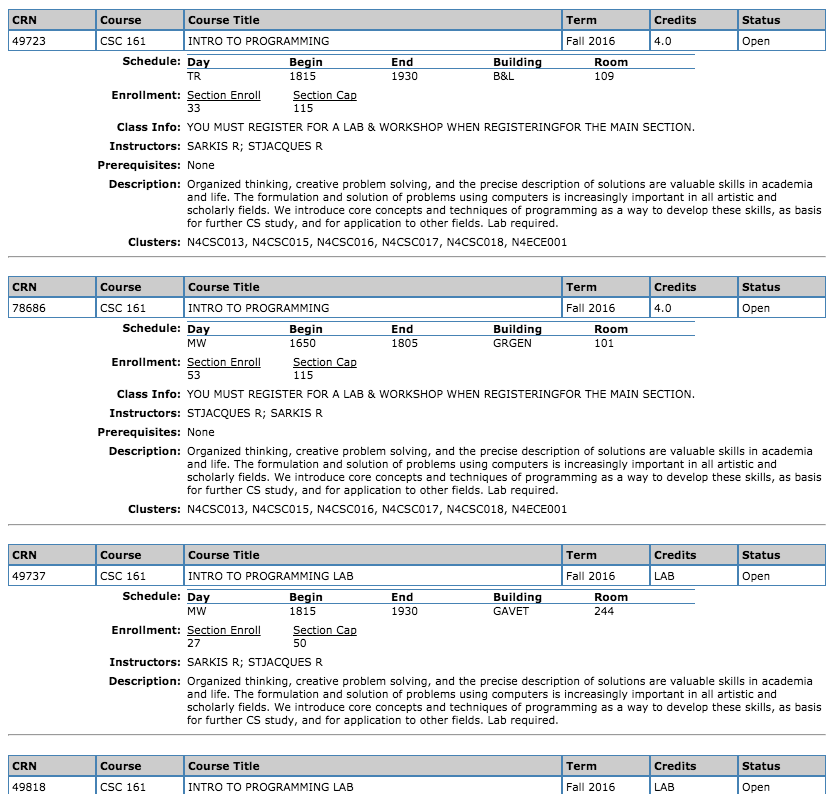
\includegraphics[width=1.00\textwidth]{images/cdcs/sections}
      }
      \caption{Ungrouped sections in CDCS} \label{fig:cdcs-sections}
    \end{subfigure}
    \hspace{15pt}
    \begin{subfigure}[h]{7cm}
      \centering
      \fbox{
        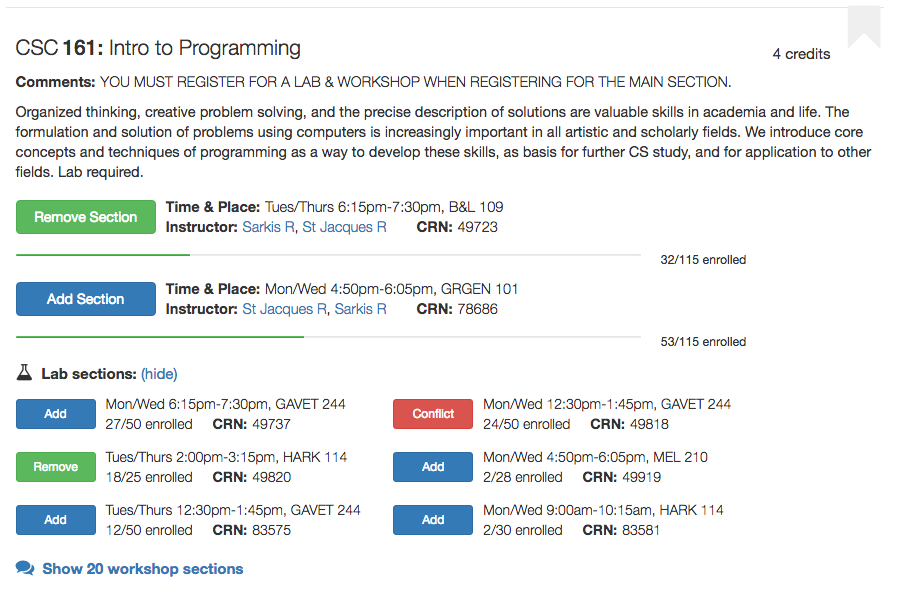
\includegraphics[width=1.00\textwidth]{images/skedge/sections}
      }
      \caption{Grouped sections in Skedge} \label{fig:sk-sections}
    \end{subfigure}
  \end{tabular}
  \caption{Section and subsection presentation in CDCS and Skedge}
\end{figure}


\subsection{Course reference}

\emph{Course mentions} will often appear in the prequisites, crosslists, comments, or description fields of a course (e.g. ``\textbf{Prerequisites:} CSC 171 or equivalent; MTH 150 is REQUIRED''). Users frequently want to find out more information about mentioned courses (frequency shown in Chapter 4). In CDCS, because course mentions are displayed as ordinary plaintext, users have to scroll back up, make a search for \emph{that} course, and lose their current search context as a result.

Skedge solves this by linking each course mention to its search query, in the style of Wikipedia. Moreover, it prevents context-switches by displaying a popover containing information on that course when the user hovers their cursor over the course mention (see Figure \ref{fig:sk-hover}).

\begin{figure}[ht]
  \centering
  \vspace{2pt}
  \fbox{
    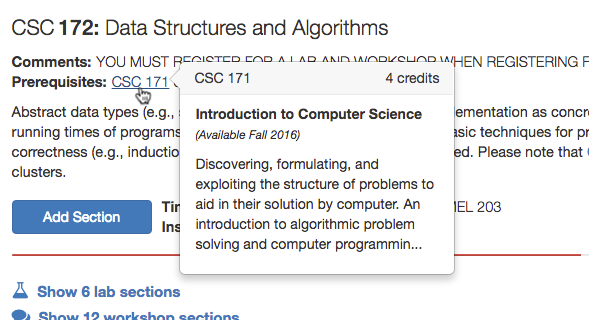
\includegraphics[width=8cm]{images/skedge/hover}
  }
  \caption{Hoverable and clickable course mention in the \emph{Prerequisites} field of a course} \label{fig:sk-hover}
\end{figure}

\subsection{Multiple schedule support}

With an active schedule still in use, students often want to plan their next semester's schedule. This is impossible with the Better CDCS extension, which instead adds courses from both terms to the same schedule, sometimes causing non-existent conflicts. A CDCS user must clear their entire schedule out before scheduling a new one. On Skedge, however, when a user adds a section of a term for which they do not yet have a schedule, a new one will automatically be created for that term. Users are also able to access their old schedules.

Additionally, a common feature request for Skedge is the implementation of multiple schedules \emph{per} term, allowing users to experiment with different schedule possibilities.\footnote{Currently under development, but simple to implement given the existing schedule management structure.}

\subsection{Schedule export}

Better CDCS provides two ways for users to export their schedule---as image or to Google calendar--except that the Google Calendar export feature is completely non-functional, telling users that ``{\tt This export tool will only work properly for the Spring of 2015}'' only \emph{after} they authorized the tool to access their Google account.

Notably missing as an export option is the \emph{iCalendar} file format (extension {\tt .ics}), which can be imported into many calendar software products. It is the only format the Mac OS and iOS Calendar applications can accept, to offer one example of very popular products that are therefore unsupported by Better CDCS.

Skedge provides the option for users to export their own or another user's schedule directly to \emph{Google Calendar} (even allowing users to choose a calendar---or create a new one for Skedge---to insert their courses into), as an \emph{image} (JPEG, PNG, or SVG), or in {\tt .ics} format (see Figure \ref{fig:sk-export}). The {\tt .ics} and Google Calendar exports include course codes, titles, locations, and properly repeat courses until the end of the current semester.

\vspace{20pt}

\begin{figure}[ht]
  \centering
  \vspace{2pt}
  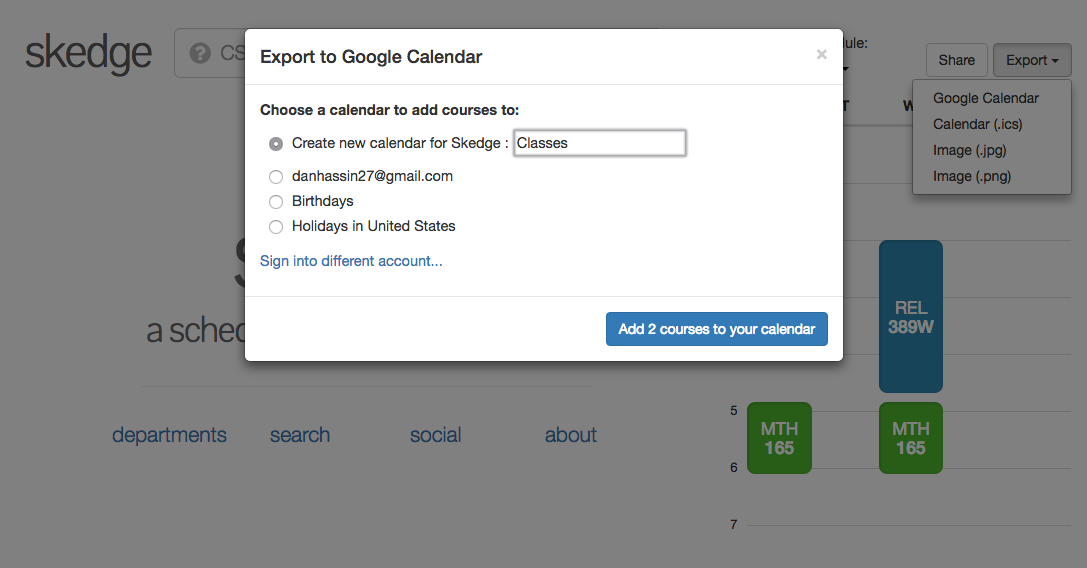
\includegraphics[width=14cm]{images/skedge/export}
  \caption{Exporting to Google Calendar (note the other export options on the top right)} \label{fig:sk-export}
\end{figure}

\clearpage